\section{Desarrollo Experimental 1}

Para empezar debemos identificar el numero del conjunto de placas que usaremos.


\begin{table}[H]
\resizebox{\columnwidth}{!}{%
\begin{tabular}{|l|l|}
\hline
Conjunto de Placas Nro: &  \\ \hline
\end{tabular}%
}
\end{table}

Ahora realizamos las siguientes conexiones.

\begin{figure}[H]
    \centering
    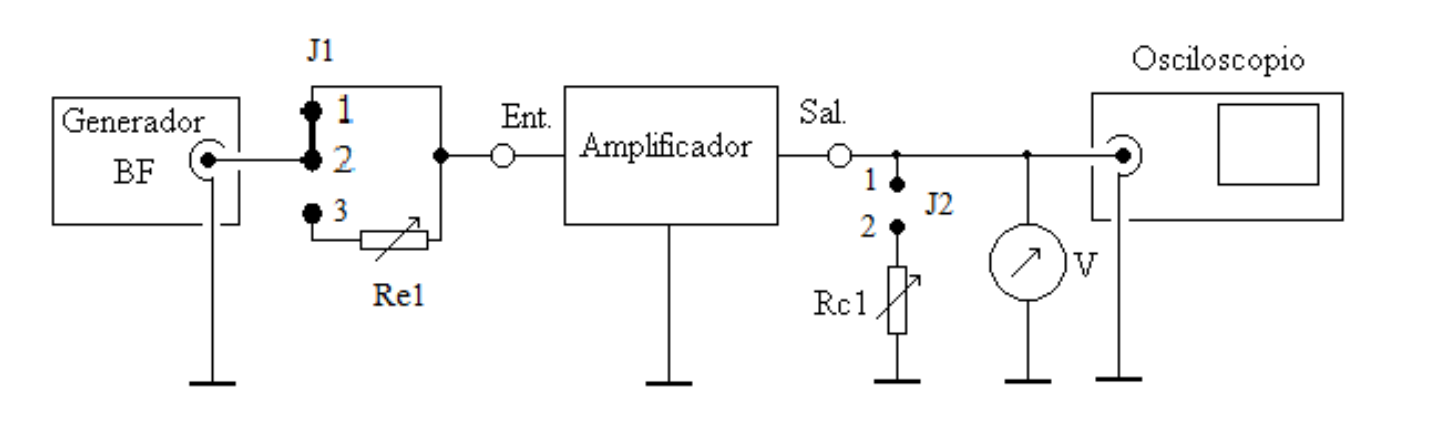
\includegraphics[width=0.5\textwidth]{images/esquema.png}
    \caption{Conexiones realizadas}
    \label{fig:conexiones}
\end{figure}

Alimentaremos el amlificador con 12V y usaremos una señal de 1KHz. La amplitud de la señal para todos los experimentos seá la máxima posible sin distorsión.\\
Ahora mediremos sin carga a la salida del amplificador y obtendremos la siguiente señal.

IMAGEN

Luego conectamos la resistencia de carga RC1 y ajustamos para que la lectura de la tension de salida se reduzca a la mitad. En este puntoi el valor de la impedancia de salida del amplificador es igual a la resistencia de carga.\\
Por lo que pasaremos a desconectar la fuente y abrir el circuito para medir la resistencia de carga. De esta forma obtenemos el valor de la impedancia de salida del amplificador.\\

\begin{table}[H]
\resizebox{\columnwidth}{!}{%
\begin{tabular}{|c|c|c|c|c|}
\hline
f1 &
  \begin{tabular}[c]{@{}c@{}}"Valor nominal" \\ de Zsal = Ro\end{tabular} &
  \begin{tabular}[c]{@{}c@{}}Vs \\ (Rc1 desconectada)\end{tabular} &
  Rc1 = Ro &
  \begin{tabular}[c]{@{}c@{}}Incertidumbre \\ de Rc1\end{tabular} \\ \hline
1KHz &
  50 ohms &
  a &
  vg &
  f \\ \hline
\end{tabular}%
}
\end{table}